\documentclass[tikz]{standalone}
\usepackage{ctex}
\usepackage{tikz}
\usepackage{pgfplots}
\pgfplotsset{compat=1.18}   % 使用较新版本语法
\usetikzlibrary{positioning, arrows.meta, intersections, calc, fit, backgrounds}
\usepgfplotslibrary{fillbetween}  % 用于填充区域
\begin{document}

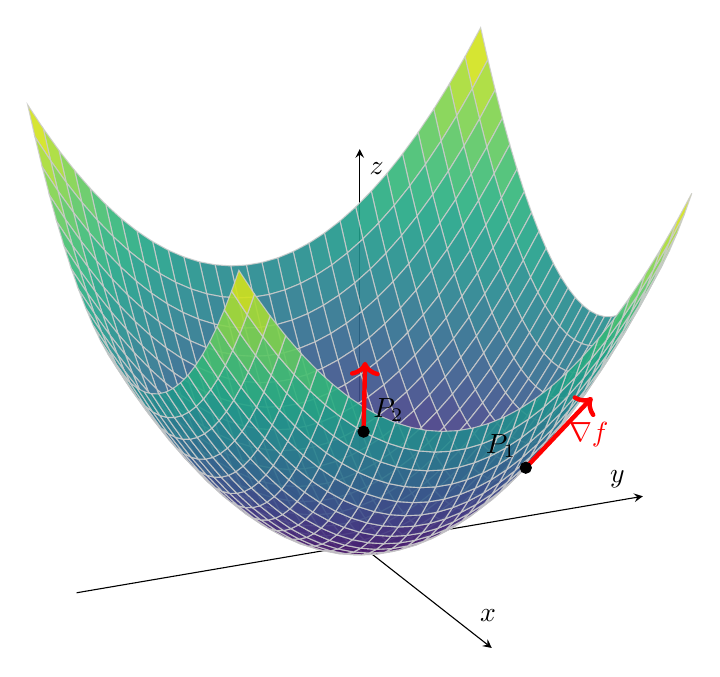
\begin{tikzpicture}
    \begin{axis}[
            xlabel=$x$, ylabel=$y$, zlabel=$z$,
            domain=-2:2, domain y=-2:2,
            view={65}{30},
            width=\textwidth,
            colormap/viridis,
            % colorbar,
            axis lines=center,
            xmin=-2.5, xmax=2.5,
            ymin=-2.5, ymax=2.5,
            zmin=0, zmax=8,
            ticks=none,
            declare function={
                f(\x,\y) = \x^2 + \y^2;
            }
        ]
        % 绘制曲面
        \addplot3[surf,
            domain=-2:2,
            domain y=-2:2,
            samples=30,
            samples y=30,
            opacity=0.85,
            faceted color=black!20,
        fill opacity=0.9] {f(x,y)};{f(x,y)};
        % ---- 点 A: (1,1) 处  z=2, 梯度=(2,2), 方向导数最大值=8, 缩放0.2倍 ----
        \addplot3[mark=*, black, mark size=2] coordinates {(1,1,2)};
        \node[above left] at (axis cs:1,1,2) {$P_1$};
        % 缩放后的梯度向量：增量(0.4,0.4,1.6) -> 终点(1.4,1.4,3.6)
        \addplot3[->, ultra thick, red, solid]
        coordinates {(1, 1, 2) (1.4, 1.4, 3.6)};
        \node[below right, red] at (axis cs:1.2,1.2,3.2) {$\nabla f$};
        % ---- 点 B: (-1, 0.5) 处  z=1.25, 梯度=(-2,1), 方向导数最大值=5, 缩放0.2倍 ----
        \addplot3[mark=*, black, mark size=2] coordinates {(-1,0.5,1.25)};
        \node[above right] at (axis cs:-1,0.5,1.25) {$P_2$};
        % 缩放后：增量(-0.4,0.2,1.0) -> 终点(-1.4,0.7,2.25)
        \addplot3[->, ultra thick, red, solid]
        coordinates {(-1, 0.5, 1.25) (-1.4, 0.7, 2.25)};
    \end{axis}
\end{tikzpicture}
\end{document}
